\documentclass[conference]{IEEEtran}
\IEEEoverridecommandlockouts
% The preceding line is only needed to identify funding in the first footnote. If that is unneeded, please comment it out.
\usepackage{cite}
\usepackage{listings}
\usepackage{amsmath,amssymb,amsfonts}
\usepackage{algorithmic}
\usepackage{graphicx}
\usepackage{textcomp}
\usepackage{xcolor}
\def\BibTeX{{\rm B\kern-.05em{\sc i\kern-.025em b}\kern-.08em
    T\kern-.1667em\lower.7ex\hbox{E}\kern-.125emX}}
    
\begin{document}

\pagestyle{plain}

\title{Mounting a Cross-Site Scripting Attack:\\Exploiting input fields on a web forum.\\
}

\author{\IEEEauthorblockN{Eddy Varela, Sean Fontellio}
\IEEEauthorblockA{Introduction to Computer Security. \\
\textit{Instructor: Daniel Barowy}\\
December 13, 2019\\
}}
\maketitle



\begin{abstract}
In this project, we built an online web forum that allows users to post security related articles. Unfortunately, we built a site with a critical security flaw. The website did not sanitize the data received from users therefore, allowing our users to post whatever kind of content they want. Our goal with this paper is to examine how easily a Cross-Site Scripting Attack (XSS) can be mounted, and how dangerous they can be if not defended against. \\

The main focus of this paper is on stored XSS attacks. More generally, we will discuss reflected XSS attacks, and other classes of XSS attacks will be supplementary material to guide the reader. By the end of the paper, we will have illustrated feasible countermeasures for our stored XSS attack and other XSS attacks.
\end{abstract}

\section{Introduction}
\begin{figure}[h]
\centering
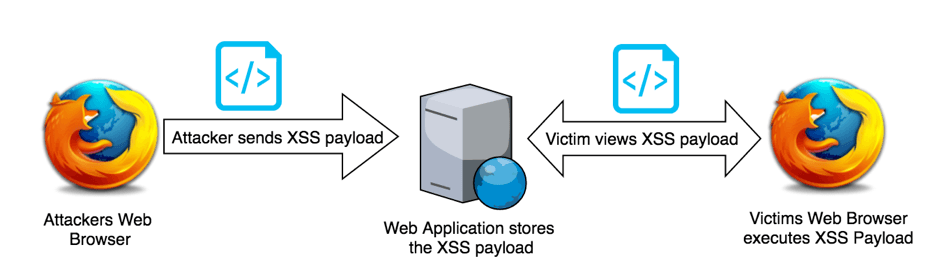
\includegraphics[width = 9cm]{stored-xss-diagram-example.png}

\caption{Stored XSS Architecture}
\end{figure}

\subsection{Cross Site Scripting Vulnerability}

``Cross-Site Scripting (XSS) attacks are a type of injection, in which malicious scripts are injected into otherwise benign and trusted websites (OWASP)." The idea behind XSS exploits revolves around developers who do not constrain the kinds of input that can be submitted on various input forms. Data that is submitted to a site is stored somewhere on a database and then rendered at later time. For example, some input forms do not restrict users from inputting malicious JavaScript code that can be executed on another browser from the server. \\ 

This trivial error has persisted as a huge vulnerability in various popular websites like MySpace, Twitter, and Facebook. In these sites, many attacks have been mounted where a malicious user can inject arbitrary JavaScript code into an application. Then, a non-suspecting user can have a different website experience or have their private information compromised. For example, suppose you had an application where people posted things for sale and the site developer did not sanitize the data that was being received. If some hacker realized this, they could potentially craft some JavaScript into the description of the object such that when a user looks at the object for sale, the hacker can gather the victim's session information (cookie that holds the data that identifies the user). The attacker is then able to impersonate this user since they have all the data that identifies that unique user.

\subsection {Variations on XSS attacks}
As XSS attacks have become more ubiquitous, defenses have also heightened in this arms race to prevent exploitation on many online sites. We will outline the variations on XSS attacks such as stored XSS, Reflected XSS, and other more exotic DOM-Based XSS attacks.\\

\subsubsection{Stored XSS}
In this variation of XSS attacks, the malicious code is stored on the server that is serving up the site. There are some limitations on this type of attack because server administrators are quickly able to find the malicious JavaScript that is causing site errors. Stored XSS is also sometimes referred to as Persistent or Type-I XSS.\\

\subsubsection{Reflected XSS}
This type of vulnerability occurs when websites reflect the same exact content back to the user on their browser without sanitizing the received data. Sanitation refers to some program logic that ensures that the input data is not malicious. This ambiguity of what can be deemed as malicious is a point of contention that makes XSS prevention quite difficult. One can imagine the realm of inputs is seemingly broad and attackers can exploit this freedom. Many XSS attacks occur when attackers inject malicious JavaScript code causing the site to behave in an unexpected way or secretly gather user data. Thus, sanitation is a non-trivial problem in XSS prevention.\\

\subsubsection{DOM-Based XSS Attacks}
The DOM is the document object model that represents all websites. The details about document object models are beyond the scope of this paper. The attack payload is executed as a result of modifying the DOM “environment” in the victim’s browser used by the original client side script, so that the client side code runs in an “unexpected” manner.
\subsection{Finding vulnerable websites}\\
To find a site that is vulnerable to cross site scripting is fairly trivial. \newline{}

1. Visit a website that accepts user input.

2. Input some JavaScript code such as: 

\begin{lstlisting}[language = JavaScript]
<script>
    window.prompt("Please enter your
    password","********");
</script>
\end{lstlisting}

3. If the site pops up a prompt asking you for your password, then the site is vulnerable to cross site scripting attacks.\\

4. Finally, this JavaScript code will be rendered to another user whenever they load the resource you are creating. Therefore, with a little more code, you can actually send their credentials onto a database.

\section{Security Assessment}\\

The resources that are compromised for sites that are vulnerable to XSS attacks are confidentiality, integrity/authorization, availability, non-repudiation. This attack is so powerful because it allows an attacker to enter malicious JavaScript that can negatively affect the website. JavaScript is powerful because it has seemingly no bounds on the kinds of information it has access to on a website. Thus, if we pair XSS attacks with a bit of social engineering, we can mount a nasty attack that negatively affects the user. A user may think this is legitimate and enter their password. With these credentials, the attacker can log in as the user given that the site does not have two-factor authentication.

\subsection{Confidentiality}
Through this attack, information that should be confidential about the user, such as their authentication tokens via cookies are at risk. Therefore, the resources that are supposed to be kept secret are quickly released to a malicious user. For example, in this attack, a malicious user input some JavaScript that simulated a page time out and requested the user's credentials to be resubmitted to a crafted URL.\\\\
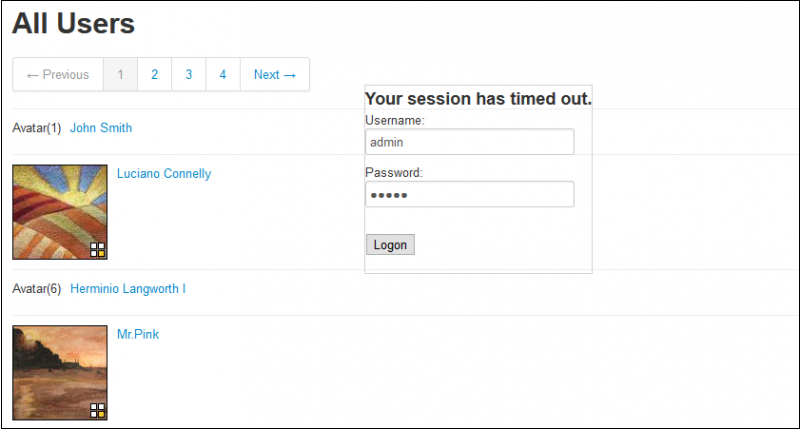
\includegraphics[width = 9cm]{xss2.png}

\subsection{Integrity/Authorization}
In general XSS attacks, integrity protection and authorization can both be compromised. For example, if we were mounting a XSS, we can try to send payments as a user who is already logged in with this script:\\

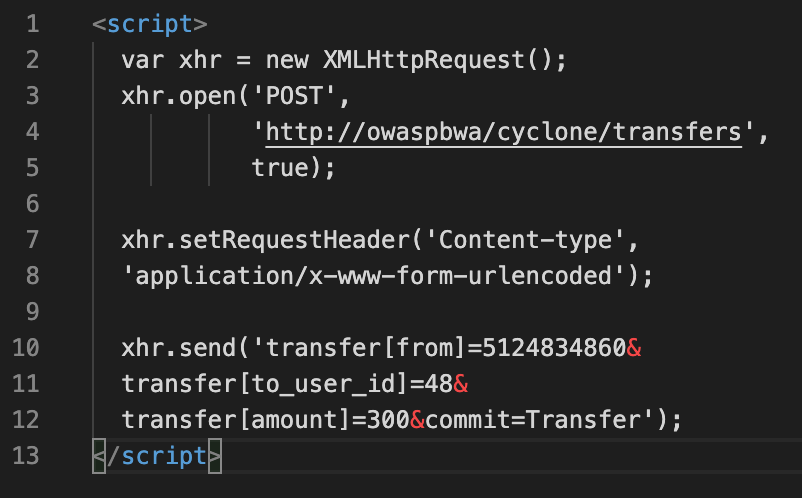
\includegraphics[width= 8cm]{ss.png}

In the previous code, the attacker opens a new connection with XHTML Request where XHTML is extensible HTML which has stricter formatting rules and error handling.\\

Then the attacker formulates a POST request which is going to make a change to database by telling the server to add a new entry of data. Namely this data entry has type 
The integrity of the user is affected because the malicious user can impersonate the victim and have full access to their account, therefore, the site is not integrity protected and authorization is not compromised. 

\subsection{Availability}
Since a malicious user can inject arbitrary JavaScript, they can essentially prevent a user from using certain features of a website. For example, someone can deface a website by placing a large image over the entire website as in this example:\\

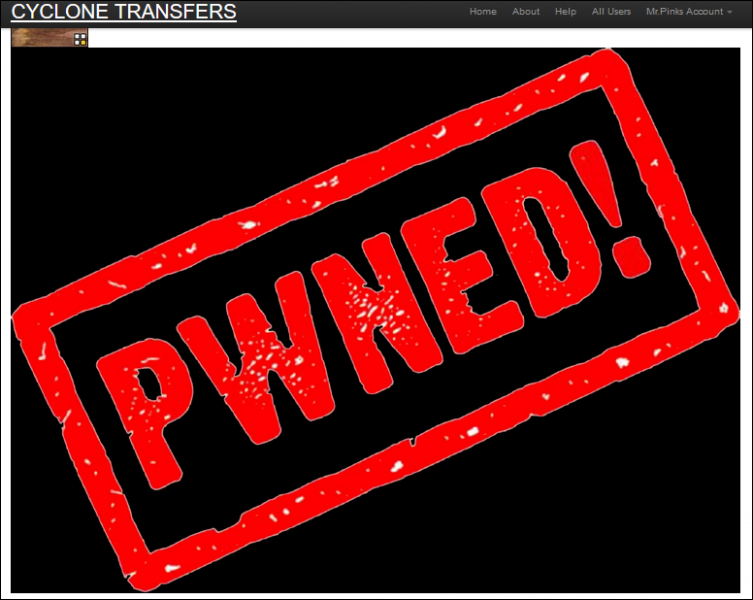
\includegraphics[width = 8cm]{xss8.png}

\subsection{Non-repudiation}

Non-repudiation is compromised because if the attacker were to do something on the victim's behalf it would be very difficult to differentiate the two.  Additionally, the attacker could utilize the user’s session id (like their unique Facebook API Key), so that their online behavior appears to be someone who it isn’t (i.e. non-repudiation). Thus, this attack affects the resources in these domains.\\

\section{Diving into XSS}

\subsection{Technical Resources}
Since this attack takes advantage of a vulnerable site, the attacker does not really need many resources except JavaScript knowledge and their own server. Alternatively, they can host a server on a popular site like AWS or Microsoft. Personally, I would not recommend this because it's not a good idea to hack on a public company's hardware and store people's sensitive information on their database service.\\

\subsubsection{Server and Database}
An attacker would need to have a server such that every request that they have mounted into vulnerable site gets handled by there server side code and stored on the database which would be hard drive.\\
\subsubsection{A vulnerable site} In order to mount this attack, the attacker must have access to a website that accepts any type of user input. Fortunately, for these attackers, there are many sites that are still vulnerable because defending against these kinds of attacks is difficult.\\
\subsubsection{JavaScript knowledge}
This is important because the domain of possibilities with JavaScript is pretty broad but one must have a decent knowledge of the language and web technologies more generally.

\subsection{Who would benefit from these attacks}\\

\subsubsection{Business Competitors}
Through XSS attacks, a competitor of a particular website could redirect users to their website or damage the reputation of the attacked website/owner. Competitors will benefit because all the traffic gets redirected to their site such that the hacker’s website is the one benefiting or gaining traction and money. The attacker could craft a fake login screen, to extract more personal and financial information from the victim. Hence, the consequences of this attack can be very severe since it is not very challenging to mount a XSS attack and can be conducted without the user or website owner being aware of the attack.\\
\subsubsection{Attackers attempting to farm user data}
If an attacker is trying to mount a more sophisticated attack, they may need to gather information from multiple places that a user is registered on. XSS is a quick and easy way to gather more information from a site that may be insecure and can be used to cross reference an email address or username.

\subsection{Is the attack difficult?}
No, in our experience, the attack is quite trivial. We purposely built a website that did not sanitize user inputs and used dangerous libraries. Exploiting these vulnerabilities took seconds after we knew that the service did not check for script tags or implement any of the various countermeasures that will be discussed later. The hard part seems to be finding vulnerable sites which would mean auditing all sites that are on the web. 

\subsection{Attack Consequences}\\
The consequence of XSS attacks can range from trivial unexpected behaviour on the target site to complete denial of service, or integrity issues, to complete access of a site. It is no surprise that this attack is one of the most popular types of web exploits (OWASP).

\subsection{History of XSS Attacks}
In the past, circa 2008, prominent social-networking sites like Twitter, Facebook, MySpace, YouTube and Orkut have been affected by XSS attacks. Since then, XSS vulnerabilities have surpassed buffer overflow vulnerabilities to become the most common publicly reported security vulnerability, with researchers estimating that as many as 68\% of websites are likely open to XSS attacks (MITRE). This attack has been deployed maliciously on the aforementioned sites to spam users, navigate them to pornographic sites, and steal sensitive information.

\section{Implementing a XSS Attack}
\subsection{How does it work?}
On a high level, we will be writing malicious JavaScript into an input field of a sandboxed website. In order to carry out any of these attacks, we must verify that a website allows user supplied javascript code to be executed on the site. Many modern frameworks have made these task tricky so we needed to work around this complication in our attack. 

For the reflected XSS attack we must send malicious JavaScript to our victim through a third party medium. Often times hackers exploit social media sites with strange link from friends or popups on other sites. After the victim has clicked on the crafted the link, they will visit the vulnerable site and execute the script that is embedded in the link. Finally, since the site is vulnerable the attacker will have compromised some sensitive data that they can use later to impersonate the victim. This attack shows a clear example where integrity, authenticity, and non-repudiation are compromised.

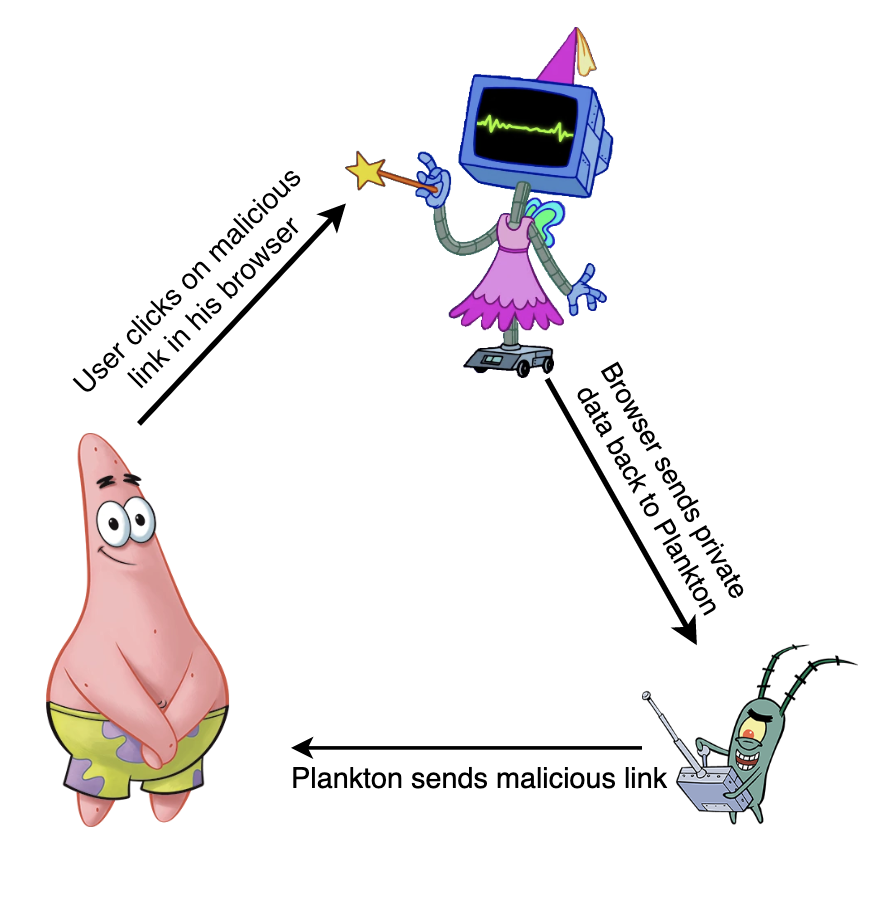
\includegraphics[width = 9cm]{reflected1.png}

For a Stored XSS attack, we will depend on the website storing our malicious script on their database. Then whenever a user loads our resource, be it a post, a picture, or some other data, the script will get executed and the attack will be successful.\\
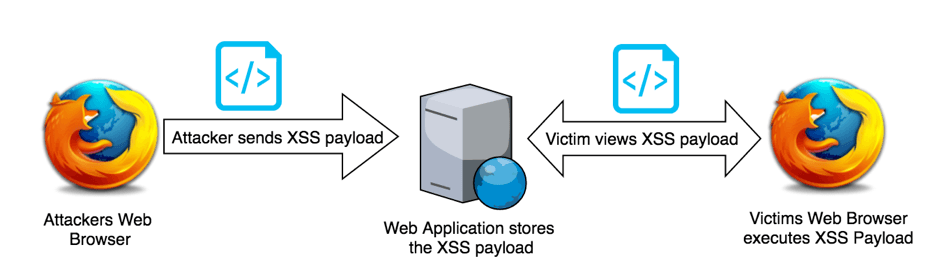
\includegraphics[width = 9cm]{stored-xss-diagram-example.png}\\

\subsubsection{Architecture}

For our attack, we built a web application on modern web development technologies like NodeJS, ReactJS, MongoDB, and Express. NodeJS is the server that handles the requests made to the application while the web interface serves up the frontend content in ReactJS. This type of attack can be carried out with any language/framework, but we chose these set of technologies to add an additional layer of difficulty. Technologies like ReactJS have several security features by design like string variables in views are escaped automatically. As a result many companies run their services on the back of these technologies. We thought it would be a challenging yet fruitful venture to exploit these frameworks.\\
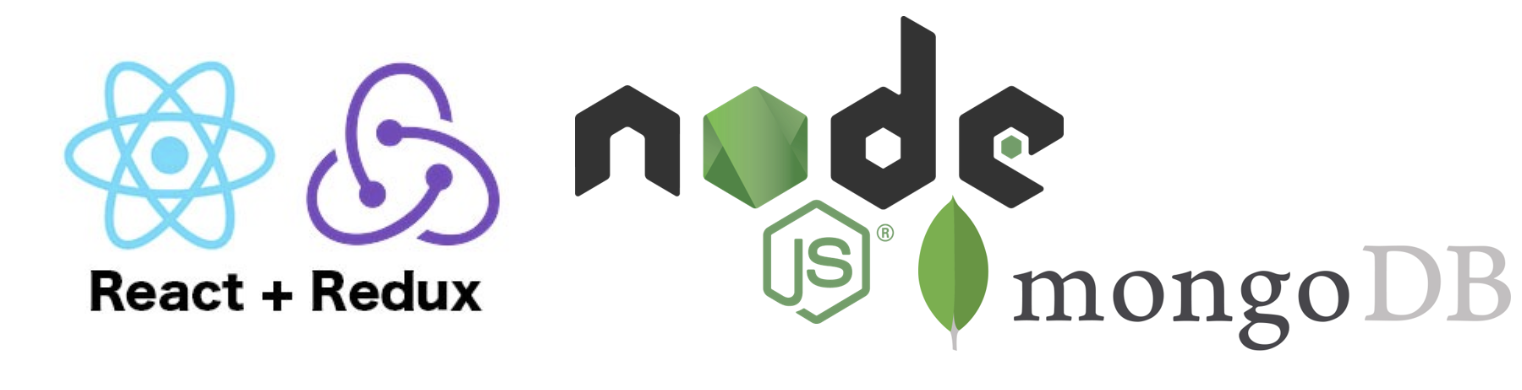
\includegraphics[width = 9cm]{architecture.png}

\section{Our Attack: Stored XSS on Hacker News}\\

HackerNews allows users to post their own articles about various discoveries in security. Then other users would navigate to a specific topic and see various articles. Unfortunately, our users have a special skill set, that is, they are clever hackers. One of our favorite white hat hackers told us exactly how to exploit this website, and walked us through how we should patch it.\\
\subsection{Mounting the attack on ReactJS}

Since React has many security features enabled by default, we will have to investigate how to carry out this attack by digging into how React works.

Components represent the basic building blocks in React and everything that is displayed on a React website are components or live within components.

This code snippet creates a React component by transpiling this code:\\

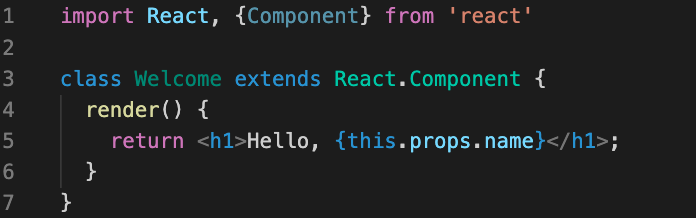
\includegraphics[width = 9cm]{reactComponent.png}\\

Into ES6 JavaScript when the app is built:\\

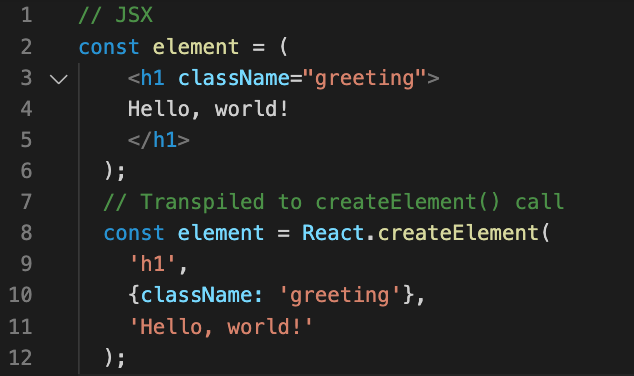
\includegraphics[width = 9cm]{jsx.png}\\

I want to direct our attention to the React.createElement() function because this is where we are going to lay the attack. This function takes in three parameters, the type of HTML tag that will be the root of DOM Tree, the props that are passed into the component, and the children which are also components. This recursive structure is built upon the tree like structure of the Document Object Model (DOM) underlying every webpage on the internet.\\


\textbf{The vulnerability: Injecting Child Nodes} ``In March 2015, Daniel LeCheminant reported a stored cross-site scripting vulnerability in HackerOne" (DailyJS Medium Article). This issue arose because the site allowed an arbitrary, user-supplied object as the children argument to React.createElement().\\
Afterwards, the code must have had some vulnerability where it fetched user supplied data and parsed it as JSON and put it into the body of the code like this :\\\\
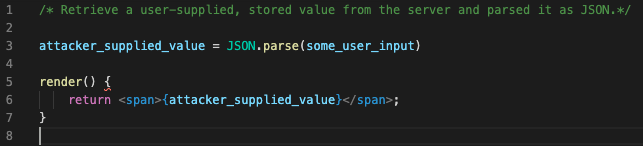
\includegraphics[width = 9cm]{JAVASCRIPT.png}\\\\
This gets transpiled into \\\\
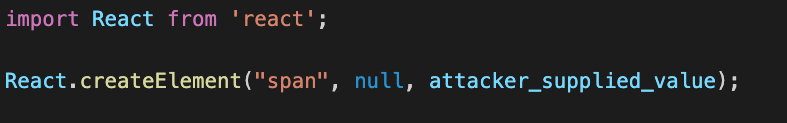
\includegraphics[width = 9cm]{TRANSPILEDATTACK.png}\\

\textbf{User supplied values for props}\\
The React developers are aware of the security vulnerabilities that result from the method setInnerHTML which allows developers to modify the HTML of web page through JavaScript therefore, they have changed the name of this method to be dangerouslySetInnerHTML because some developers may still want to modify the HTML page with some user supplied script however the React designers want developers to \textit{know} that this is a \textbf{dangerous} method, we will exploit it.
\subsection {Attack Code}

1. First, we need a component that takes in some user supplied props. This will be our theoretical buffer such that we can inject any kind of malicious JavaScript into the program. In our project, we load in a post object and pass in their title and body into a PostView component.\\\\
On the application we have a modal that accepts user input:\\\\
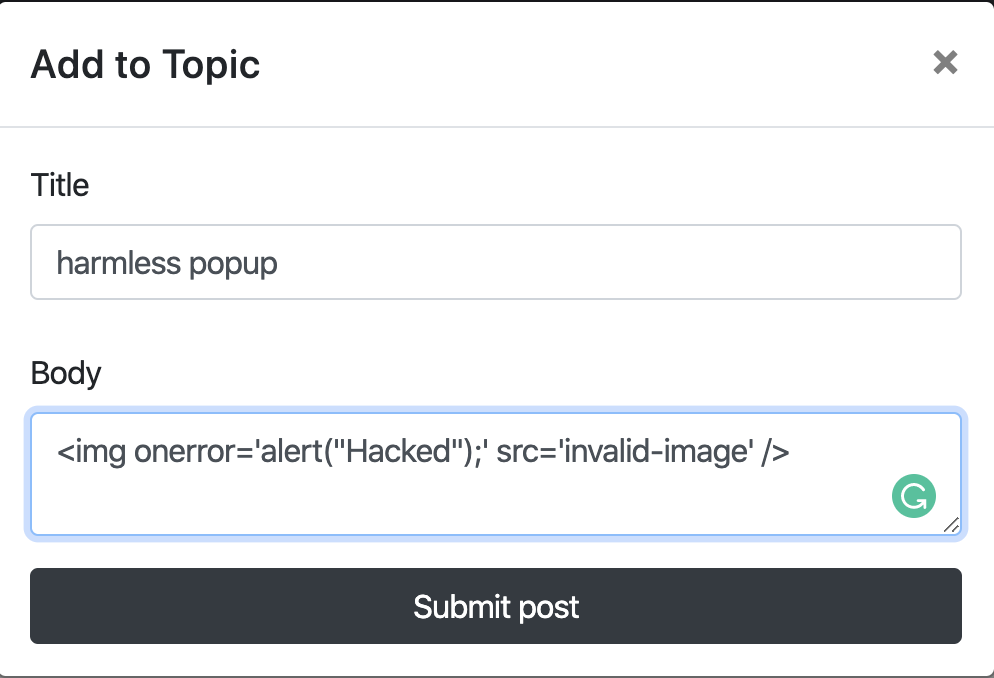
\includegraphics[width = 9cm]{modal.png}

2. Then we need a method that dangerously sets the inner HTML based on the user supplied props.\\

On the application side we see a popup that was injected by the body of user's post:\\\\
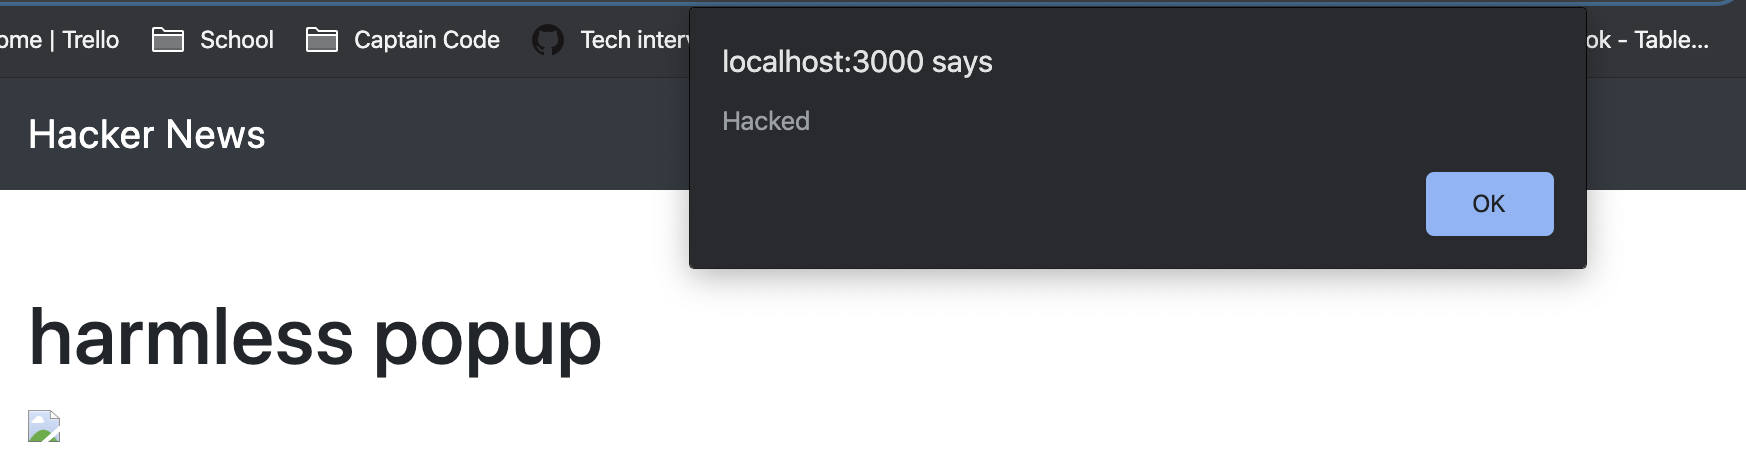
\includegraphics[width = 9cm]{post.png}\\
In the code we have a paragraph tag that runs dangerouslySetInnerHtml() with the user supplied content.\\\\
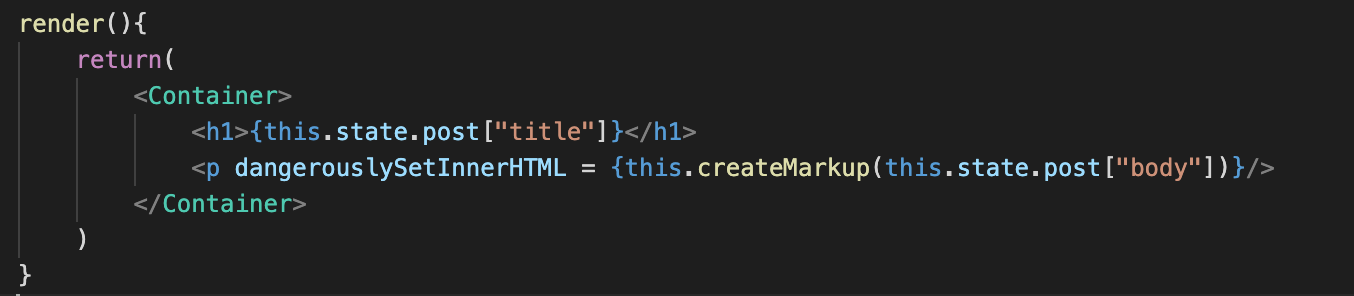
\includegraphics[width= 9cm]{buffer.png}\\
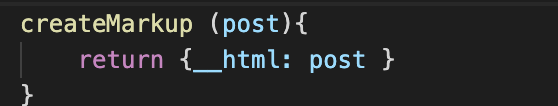
\includegraphics[width = 9cm]{method.png}\\\\
3. Finally, the script will be executed on the client side when the page is loaded.\\\\
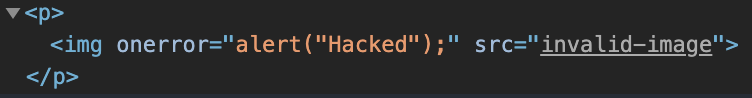
\includegraphics[width = 9cm]{inspector.png}
This is what we see from the inspector after every the post has been loaded up.

\subsection{Defenses:}

There's not a well known algorithm to prevent this kind of attack especially when the user is allowed to write raw HTML and JavaScript code into the inputs. Therefore, there are several libraries and paradigms that make XSS attacks more difficult. For example, one popular library is jsxss, a sanitizing library for JavaScript applications that take in untrusted HTML.\\

When building React applications, avoid using dangerouslySetInnerHTML whenever possible. When it is impossible to avoid this method, sanitize in all layers and then render the HTML.

\subsection{Severity and Likelihood}\\
As described in the Security Audit section, the severity of this attack is extremely dangerous as it can affect resources in all different domains outlined before. The likelihood of an attacker mounting a successful attack is the probability that they are able to find a site that is vulnerable to XSS attacks. Once they can find the site, they're guaranteed to mount an attack.
\section{Countermeasures:}

As for countermeasures, there are many best practices to follow to decrease the likelihood of a XSS attack. The underlying tenet of these preventative measures is skepticism. As a developer you must believe that all data not produced by you is malicious. Anything that comes from outside one's system like form data, query strings, cookies, request headers, etc should not be rendered on a webpage. Many developers forget this and allow different forms of attacks like SQL injections, XSS, and other malicious user input attacks.\\
Many language designers have baked in character escaping such that scripts get rendered out as plaintext. For example, the React framework we used to build HackerNews has character escaping whenever it encounters angle brackets like <script>, <h1>, etc. However, as we have shown there are still instances where developers use dangerous methods like dangerouslySetInnerHTML. Although this method has an alarmingly insecure name, developers may not know why it’s dangerous. Therefore, as developers, we must be cautious of the kind vulnerabilities that we can introduce into the apps we build. A good countermeasure is to be informed of existing vulnerabilities.

\subsection{Sanitizing inputs}

Although it may see like sanitizing inputs is simple enough, there are many technical challenges which we will have to account for. Luckily, there are several libraries and resources to assist developers in building sites that are less vulnerable.\\

\subsubsection{Whitelisting}\\

As a countermeasure for malicious user input, developers can either whitelist or blacklist the content that is being received. Whitelisting is the process of describing everything that is understood to be non-malicious and allowing this type of content to get stored in the app. On the other hand, blacklisting refers to identifying malicious kinds of input and rejecting this data from our application. The challenge with this approach is that some sites allow users to submit HTML and JavaScript. It is difficult to write an algorithm that prevents any kind of malicious input and handle encoded data. Therefore, many prefer whitelisting as it is easier to decide what is non-harmful.\\ 
\subsubsection {Form Validation}
Developers can type check the data that they are receiving. For example, if a developer expects a user to enter their height, they should not be submitting a script or text into this field. This is a fairly simple countermeasure but can go a long way.\\
\subsubsection{Layered approach}
Many developers recommend sanitizing inputs on every layer. This would prevent a man in the middle attack. Suppose the web application sanitizes inputs on the front end but does not do any explicit checks in the backend. A malicious user may be able to intercept a packet and modify it such that the content gets stored in the database without the developers even knowing.\\
\subsection{Update Libraries}
Keep the latest patches on software as many times, hackers find creative ways to exploit different systems. Furthermore, don't use libraries that are known to be dangerous. Many libraries will exist to support legacy applications but if they can be avoided please do so at all costs. If you are maintaining an application with risky libraries and method calls, just remove them and patch your software.\\
\subsection{Pentesting}
Test the security of your system frequently. As software grows, there are many places where hackers can try to find an opening. Make sure that your organization can find it before the hackers do.

\subsection{Best Practices in Development} 
Avoid URLs that explicity have some reference to JavaScript or JavaScript code. 

Do not use untrusted third party applications as they may not be reliably protecting against XSS attacks. Try to prevent users from inputting data into these third party applications that may store the information onto your database. This could be catastrophic for your entire application.

\section{Conclusion:}

Security vulnerabilities and destructive users trying to hijack or attack a program will persist. Even in the last couple years, technology and security practices have drastically changed. Not to mention, the growing trend of incorporating technology anywhere and everywhere possible. Cross-site scripting attacks will continue to exist for a long time due to their ease of implementation and the underlying structure of how sites communicate between a server and a database. The way in which websites are constructed such that a server displays the content for every request. When it comes to feeling secure, trust is one of the most essential values in relationships or vital when it comes to sensitive information. However, trust can never fully be established between a user and an online interfaces; all web pages are technically vulnerable to XSS attacks. This means that it is nearly impossible for a random user to discern which aspects of the site were originally implemented by the developer and which ones were potentially placed there by a hacker. Additionally, an attacker might pair this attack with other attacks, such as logic bombs, (D)DOS, or privilege escalation.  If they do such a complex attack like this then they are able to run scripts in the background of your browser without your awareness, and steal information whenever they want after a time detonation, or through “shortcutted” executive access. In conclusion, this attack is harmful and defenses against XSS attacks should be considered prior and throughout the process of setting up a website. Otherwise, negative consequences can result which will hinder proper functioning of the web domain and have user data open to malicious activities.

\end{document}
